\part{Fundamentos da Comunicação por Luz Visível}

\chapter[HISTÓRICO]{História do VLC}

Existem relatos da luz sendo utilizada com a finalidade de comunicação sem fio antes
dos anos 800 A.C. Fogueiras eram acesas e utilizadas como um farol para sinalizar,
 assim como sinais de fumaça para realizar comunicações a longa distância. A luz do sol 
 já foi utilizada combinada com espelhos para enviar luz direcionada a um local especifico, realizando sinalizações. 
 Nos século XIX lâmpadas eram usadas para comunicação entre barcos e faróis para 
 alertar as embarcações de perigos, condições das águas e até mesmo bancos de areia.\\

Apesar da luz ter sido utilizada desde a antiguidade para transmitir informações a longas distâncias, o sistema de comunicação era capaz de transmitir apenas um único bit de informação, e isso era de longe o meio mais rápido de transmitir informações sobre eventos importantes a localidades afastadas.\\

Nos começo do anos 1790, Claude Chappe inventou o telégrafo óptico, o qual era capaz de enviar mensagens a longas distâncias mudando a orientação do \lq\lq braço\rq\rq \: sinalizador provido de espelhos em uma torre. Um livro com orientações de sinalização foi criado para codificar letras do alfabeto, numerais e palavras comuns. Essas mensagens podiam ser enviadas a distâncias da ordem de quilômetros em questão de minutos.\cite{Standage:1998}

Um dos primeiros sistemas de comunicação óptica a utilizar detectores eletrônicos foi o fotofone criado por Graham Bell e Charles Tainter, este dispositivo foi patenteado em 14 de dezembro de 1880, nos Estados Unidos da América.\cite{Azzawi} 

\begin{figure}
	\centering
	\label{Desenho do fotofone por Alexander Graham Bell e Charles Tainter}
		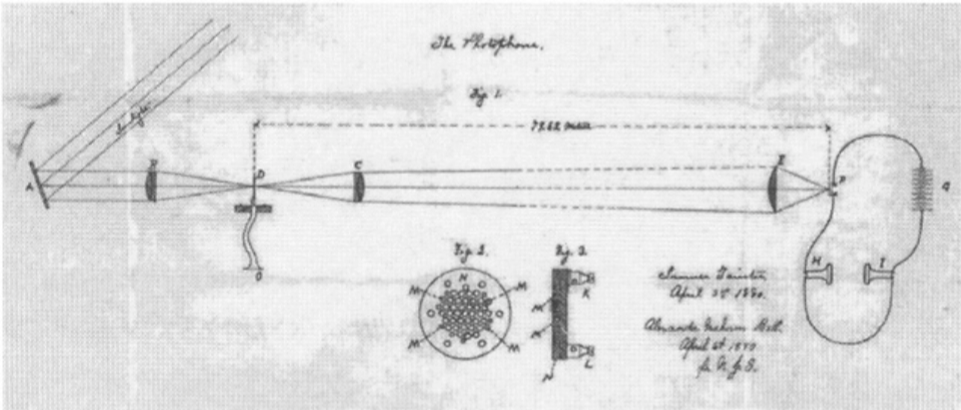
\includegraphics[width = 12cm]{figuras/fotofone}
	\caption{Desenho do fotofone por Alexander Graham Bell e Charles Tainter \cite{Hranilovic}}
\end{figure}

A figura [\ref{Desenho do fotofone por Alexander Graham Bell e Charles Tainter}] apresenta o desenho do dispositivo feito pelos criadores. O sistema foi projetado para transmitir a voz do operador a distância pela modulação da luz do sol que refletia em um diafragma. Do outro lado o receptor consiste de um cristal de selênio que converte o sinal óptico em corrente elétrica. Com este aparato, os criadores eram capazes de transmitir sinais de áudio a uma distância de 213 metros. \cite{Fotofone}

A era moderna de comunicação óptica indoor iniciou em 1979 por F.R. Gfeller e U. Bapst com o uso de transmissões difusas na faixa de infravermelho para comunicação óptica de médio alcance.\cite{Gfeller}


\section{Meios de Comunicação sem Fio}

Atualmente a maioria dos dispositivos wireless fazem o uso das faixas de frequência ISM.
A banda ISM compõe parte do espectro de rádio que pode ser utilizada para basicamente qualquer proposito sem a necessidade de requerer licença na maioria dos países. Nos Estados Unidos da América as faixas de banda 902-928 MHz, 2.4 GHz e 5.7-5.8 GHZ eram inicialmente utilizadas para maquinário que emitiam rádio frequência como fornos micro-ondas e máquinas de solda, mais não para comunicação via rádio.
Com o passar dos anos as regulamentações mudaram e as faixas de RF que antes eram desperdiçadas agora fazem parte de uma das frequências mais utilizadas para na telecomunicação.

\begin{table}[h]
	\centering
	\begin{tabular}{cc}
		\toprule
		\textbf{Bandas ISM} & \textbf{Limite de Potencia (Watts)} \\
		\midrule
		\textbf{902 - 928 Mhz} &  \\ \hline
		Telefone sem Fio & 1 W\\
		Forno microondas & 750 W \\
		Aquecedores Industriais & 100 kW\\
		Radares Militares & 1000 kW\\ \hline
		\textbf{2.4 - 2.4835 Ghz}&  \\ \hline
		Bluetooth & 100 mW\\
		Wi-Fi - 802.11b/g & 1 W \\
		Forno microondas & 900 W\\ \hline
		\textbf{5 GHz} & \\ \hline
		5.725 - 5.825 GHz & 4 W\\
		Wi-Fi - 802.11a/n/ac & 4 W \\
		\bottomrule
	\end{tabular}
	\caption{Frequências utilizadas pelos dispositivos de comunicação RF wireless padrão \cite{ISM}}
	\label{Tab: frequencias RF}
\end{table}

Na tabela [\ref{Tab: frequencias RF}] são apresentadas os protocolos e dispositivos que usufruem da bada ISM. Estão presentes na lista dispositivos militares e industriais, e também dispositivos muito utilizados no nosso dia a dia como é o caso da tecnologia Bluetooth, IEEE 802.15, e do Wi-Fi, IEEE 802.11. 

O Bluetooth é  um das tecnologias mais populares de WPAN, Wireless Personal Area Network, e pode ser encontrado na maioria dos telefones portáteis atuais. 
Sendo uma tecnologia que atua em na área pessoal de comunicação ponto a ponto, a tecnologia bluetooth substitui conexões físicas de diversas maneiras, como por exemplo telefone celular e headsets e monitores cardíacos e equipamento medico.\cite{1368913}
Hoje a distância de cobertura pode alcançar os 50 metros com a tecnologia Bluetooth 4.0. \cite{Bluetooth}

Já o protocolo de comunicação Wi-Fi é destinado ao uso em WLAN, Wireless Local Area Network. Como a área de cobertura do Wi-Fi é maior, dispositivos portadores desta tecnologia são utilizados em escritórios, escolas e laboratórios podendo conectar dois ou mais dispositivos dentro da área de cobertura.

Com o uso de tantos dispositivos sem fio a banda ISM se encontra congestionada. Em prédios residenciais e escritórios vários modems disputam por um dos canais de comunicação disponíveis, e quando não o encontram o resultado é a interferência dos sinais e impossibilidade da comunicação do host com o modem.

\subsection{VLC vs. Radiofrequência}

Como o número de usuários que utilizam comunicações por radiofrequência tem aumentado consideravelmente nos últimos anos. Isso graças ao crescimento e avanço na tecnologia dos celulares e popularização das redes Wi-Fi. Os serviços de comunicação sem fio se tornaram indispensáveis, porém este sistema ainda apresenta algumas desvantagens.

Um do grandes problemas é a capacidade. O espectro de rádio é relativamente pequeno, e seu uso é limitado e ainda o seu licenciamento é caro. A comunicação Wi-Fi disputa parte da banda ISM, apresentado na tabela [\ref{Tab: frequencias RF}], com outros dispositivos eletrônicos como telefones sem fio e fornos microondas. Por este fato podemos constatar que a bada dedicada a esta comunicação está congestionada.\cite{boucheto.2006} Como possível solução, podemos utilizar o espectro de luz visível. O VLC é uma modalidade de comunicação sem fio onde os dados são modulados na porção de luz visível do espectro eletromagnético, que compreende a faixa de comprimento de onda dos 380 nm aos 780 nm aproximadamente, apresentado na figura[\ref{Fig: espectro-visivel-da-luz}]. Com o VLC problemas de interferência por radiofrequência são minimizados.
Se comparado o tamanho do espectro de luz visível com o espectro de ondas de rádio, percebemos que o espectro de trabalho do VLC é muito maior. Fato que garante maior largura de banda de transmissão.

\begin{figure}
	\centering
		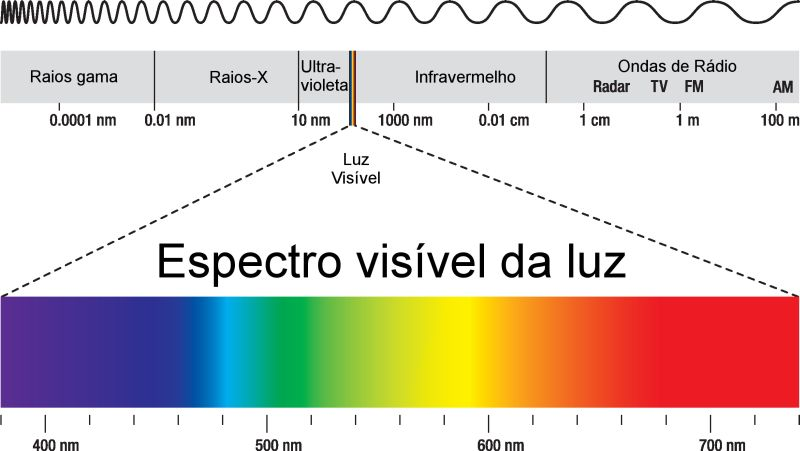
\includegraphics[width = 12cm]{figuras/espectro-visivel-da-luz}
	\caption{Espectro de luz visível ao ser humano.}
	\label{Fig: espectro-visivel-da-luz}
\end{figure}


O VLC é o tipo de tecnologia do futuro, pois busca agregar em um só produto a economia de energia com o uso de lampadas LED, que são energeticamente eficientes, com o envio de dados em altas taxas de transmissão. Sem contar o fato de que o custo de investimento no design de um sistema VLC é muito menor quando comparado aos sistemas de RF.

É sabido que existe o problema de disponibilidade de ondas de RF. Visto que em certas situações não é recomendado utilizar ondas de rádio, como em voos e hospitais. Pois o mesmo pode gerar interferência em outros aparelhos. Nestes casos podemos usar o VLC onde é necessário que haja iluminação do ambiente e ainda a comunicação de aparelho sem que haja interferência com sistemas baseados em radiofrequência. Há também o fator de segurança, já que ondas de rádio atravessam paredes e podem ser detectadas em uma vasta área. O VLC transmite dados até onde a luz alcança, se o sistema de comunicação estiver confinado em uma sala, os arredores e salas vizinhas não terão qualquer informação sobre a rede VLC.

\begin{table}[h]
	\centering
	\begin{tabular}{ccc}
		\toprule
		\textbf{Propriedade} & \textbf{Óptico} &
		\textbf{Rádio}\\
		\midrule
		Custo & \$ & \$\$\\
		Design de circuito RF ? & Não & Sim\\
		Faixa regulamentada & Não & Sim\\
		Taxa de transmissão & 100 Mbps & 10 Mbps\\
		Segurança & Alta & Baixa\\
		Passa através de paredes ? & Não & Sim\\
		\bottomrule
	\end{tabular}
	
	\caption{Comparação entre transmissão via rádio e óptico \cite{Hranilovic}}
	\label{Tab: Rádio vs VLC}
\end{table}

Em suma a utilização da radiofrequência permite a comunicação indoor e conexões de pequena distância sem a necessidade de cabos. Contudo essa solução continua relativamente cara e permite apenas médias taxas de transmissão como mostrado na tabela [\ref{Tab: Rádio vs VLC}].  As faixas de frequência utilizadas pelas conexões de RF são regulamentadas, e essas regulamentações variam de 
país para país, fazendo com que estabelecer um padrão seja difícil. Adicionalmente, a natureza das comunicações RF permitem conexão móvel, porém cria problemas de interferência entre dispositivos próximos ao transmissor. A contenção de energia eletromagnética em frequência de rádio ainda é difícil, e se esta contenção for feita de maneira inapropriada pode impedir a performance do sistema.

\subsection{Aplicações}

As aplicações do sisteme de comunicação optico sem fio são as mais variadas. Nesta seção foram organizadas as aplicações de um VLC de acordo com o alcance da transmissão. Para mostrar a versatilidade desse sistema podemos aplicá-lo na comunicação entre circuitos integrados, CIs na ordem de milímetros, e até mesmo na comunicação entre satélites, na ordem de dezenas de quilômetros como mostrado na figura [\ref{Fig: faixas-de-alcance}].

\begin{figure}
	\centering
		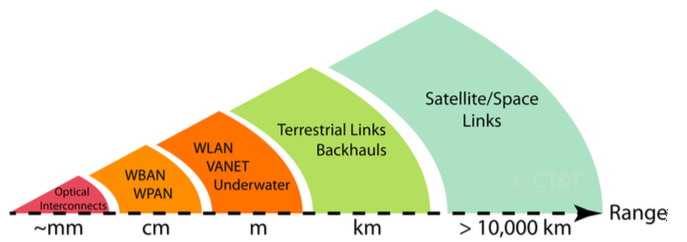
\includegraphics[width = 10cm]{figuras/faixas-de-alcance}
	\caption{Categorias de comunicação óptica baseado no alcance de transmissão.}
	\label{Fig: faixas-de-alcance}
\end{figure}

\subsubsection{Alcance Ultra Pequeno (Ultra-Short Range)}

Atualmente estão sendo estudados meios de facilitar a transferência de dados dentro de circuitos integrados e circuitos impressos. Diante da grande complexidade dos circuitos e necessidade cada vez maiores de altas taxas de transmissões em barramentos, cientistas buscam fazer comunicação de barramentos via transmissores ópticos o que pode reduzir a complexidade das vias de cobre e aumentar a eficiência na troca de dados.
Esta tecnologia trabalha na ordem dos milímetros, e esse tipo de sistema geralmente é encontrado no nível de chip, utilizado para comunicar circuitos figura [\ref{Fig: ultra-short}] ou fazer comunicação dentro de um mesmo chip. Com o uso deste meio de transmissão rápida, conexões baseadas em cobre serão substituídas. Este processo oferece benefícios na redução da latência dos dispositivos, ou seja o tempo de resposta do circuito será reduzido. Sistemas nesse nível podem ser guiados ou não. Arquiteturas  guiadas promovem um link direto de luz entre o transmissor e o receptor, confinando a luz em uma guia de onda. Enquanto nos sistemas não guiados o feixe de luz é exposto ao ambiente, o que pode causar ruídos e interferências na comunicação.\cite{c.kachrisk.bergmankereni.tomkos2013}

\begin{figure}
	\centering
		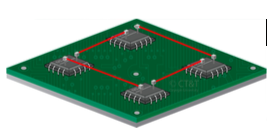
\includegraphics[width = 9cm]{figuras/ultra-short}
	\caption{Ilustração de um sistema de comunicação de pequeno alcance.}
	\label{Fig: ultra-short}
\end{figure}

\subsubsection{Pequeno Alcace (Short Range)}

Sistemas de curto alcance operam na ordem de centímetros e em geral menos que um metro. Este tipo de comunicação pode ser comparada com o Bluetooth, pois atua na mesma faixa de alcance. Uma situação comum de uso desse tipo de comunicação seria em uma rede Wireless Personal Access Networks (WPAN), assim como em uma rede Wireless Body Access Networks (WBAN). É importante ressaltar que a tecnologia infravermelho geralmente é usada nesse caso, o que não exclui a possibilidade de utilizar a tecnologia VLC. Um exemplo de aplicação desse tipo de sistema se dá em WBAN para hospitais. Centros de saúde  podem eliminar todos os fios que são conectados ao paciente com o uso da tecnologia de comunicação sem fio em aparelhos como medidores de pressão arterial, sensores de glicose, frequência cardíaca entre outros sensores de aquisição de dados figura[\ref{Fig: short}].

\begin{figure}
	\centering
		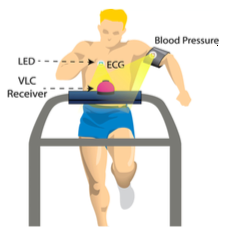
\includegraphics[width = 7cm]{figuras/short}
	\caption{Simulação de um teste de estresse cardíaco com base em um VLC. LEDs conectados as transmissores enviam dados ao receptor localizado na barra de apoio do equipamento.}
	\label{Fig: short}
\end{figure}

Pesquisas recentes nesta área incluem aplicaçoes que utilizam a câmera de celulares para recepção de dados, onde o sensor integrado, que é um sensor de imagem, é utilizado como detector óptico para a comunicação. O que permite vários tipos de transferencia de dados, como exemplo entre celulares, entre celular e televisão, celular e maquinas de auto-atendimento dentre outros.\cite{c.danakism.afganig.poveyiunderwoodh.haas2012}


\subsubsection{Médio Alcance (Medium Range)}

A comunicação indoor ,WLAN assim como o Wi-Fi, se encontra dentro do sistema de comunicação de médio alcance. Esses sistemas estão sendo desenvolvidos para que possam ser utilizados no espectro de luz visível conhecido como Visual Light Optical Communication (VLC). Por alcance médio definimos sistemas de comunicação com transmissão na ordem de metros, porém geralmente menores que 10 metros. A tecnologia vindoura nessa área é muito promissora devido aos benefícios que esse tipo de comunicação oferece. Como exemplo longa vida de duração, visto a vida útil de um LED, alta tolerância a umidade, baixo consumo de energia devido ao grande avanço na tecnologia de fabricação dos diodos emissores de luz.
As novas gerações de LEDs devem substituir lâmpadas incandescentes e fluorecentes gradativamente devido a sua capacidade de iluminação com baixo consumo de energia. A tecnologia VLC conta com a onipresença de infraestrutura de iluminação baseadas em LED para o seu sucesso.

A figura [\ref{Fig: medio1}] apresenta um sistema fixo de VLC. A luminária de mesa funciona como um modem Tx e o dispositivo USB como um receptor.

\begin{figure}
	\centering
		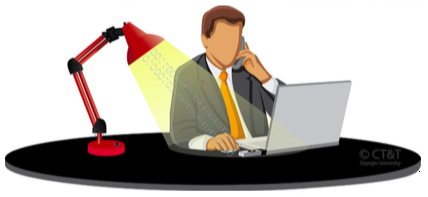
\includegraphics[width = 7cm]{figuras/medio1}
	\caption{Um hot spot VLC, onde a luminária funciona como um transmissor e o dispositivo USB como um receptor do sinal.}
	\label{Fig: medio1}
\end{figure}

Além de aplicações indoor, LEDs estão sendo vastamente utilizados em áreas abertas, para sinalização de tráfego, faróis e lanternas veiculares. Isso favorece a implementação de comunicação entre veículos, assim como automóveis e infraestrutura fixa de comunicação. \cite{Vehicle}

Veículos que possuem LEDs em faróis e lnatarna podem se comunicar com os carros próximos a ele, e com a infraestrutura, fixa nas rodovias como apresentado na figura [\ref{Fig: medio2}].

\begin{figure}
	\centering
		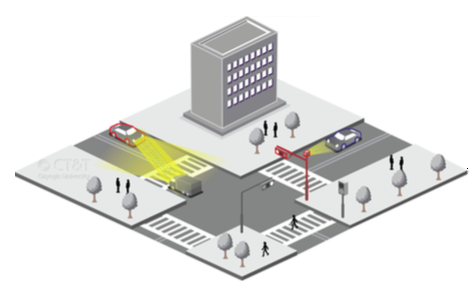
\includegraphics[width = 7cm]{figuras/medio2}
	\caption{Rede VLC veicular, veículos se comunicam entre si e com a infraestrutura fixa na rodovia.}
	\label{Fig: medio2}
\end{figure}


\subsubsection{Longo Alcance (Long Range)}

Sistemas de longo alcance operam na ordem dos quilômetros, porém não mais do que 10 quilômetros figura[\ref{Fig: longo1}]. É utilizado em geral em redes Wireless Metropolitan Access Networks (WMAN) que estão sendo desenvolvidos usando Free Space Optical Communication, que nada mais representa o não confinamento do luz.
Em comparação com o RF, uma conexão óptica FSO, possui maior largura de banda, pode chegar a taxas de transferência de dados de até Tbps. \cite{g.parcaa.shahpariv.carrozzog.tossia.j.teixeira2008}
Sistemas FSO tem chamado a atenção como uma solução eficiente de conexão entre o usuário final e a infraestrutura de fibra óptica.

\begin{figure}
	\centering
		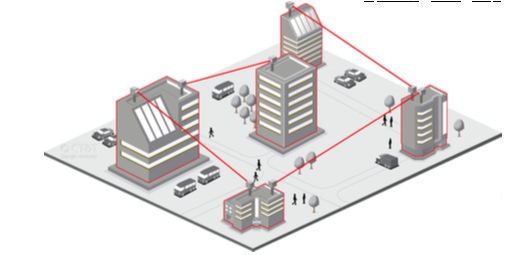
\includegraphics[width = 7cm]{figuras/longo1}
	\caption{Conexão entre prédios.}
	\label{Fig: longo1}
\end{figure}

A comunicação wireless óptica de longo alcance também tem sido projetada para que possa ser aplicada a aeronaves figura [\ref{Fig: longo2}], e nesse quesito a maior diferença está no fato de que tanto o receptor quanto o transmissor podem estar em movimento. Para que haja uma comunicação eficiente devem ser adicionadas ao sistemas dispositivos de rastreamento para localizar o destinatário desejado com o uso de algoritmos de posicionamento. \cite{Haan}

\begin{figure}
	\centering
		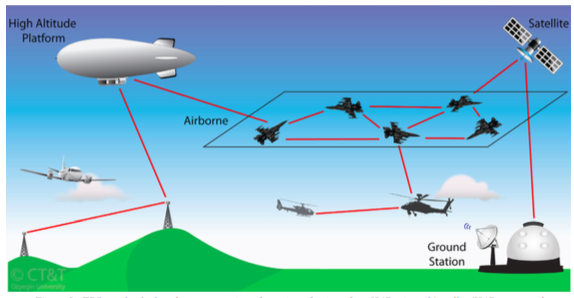
\includegraphics[width = 7cm]{figuras/longo2}
	\caption{FSO podem ser utilizados na comunicação aérea.}
	\label{Fig: longo2}
\end{figure}


\subsubsection{Alcance Ultra Longo (Ultra-Long Range)}

\textit{Ultra-Long Range} OWC faz o maior salto dentre as diferentes classificações de alcance. Esses sistemas são projetados para comunicar entre uma estação base e um satélite, de satélite para satélite ou até mesmo de planeta a planeta! O FSO nesta classificação trabalha com distâncias na ordem das dezenas de milhares de quilômetros. Em outubro de 2013, a agência espacial Norte Americana NASA com seu \textit{Lunar Laser Communication} alcançou a taxa de transmissão de 622 Mbps entre a Terra e a Lua. Ou seja atingimos a faixa de mega bits por segundo de transferencia a distância de 384 600 quilômetros entre o Tx e Rx.\cite{NASA}



\subsubsection{Sistema VLC indoor}

Até o final dos anos 90, a maioria dos Óptical Wireless Communication era feita através da comunicação no espaço livre (FSO) a qual era operada essencialmente no espectro infravermelho das ondas eletromagnéticas. Até que finalmente nos anos 2000 foi desenvolvida e implementada a tecnologia VLC, comunicação por luz visível. A faixa de luz visível ao ser humano fica entre os comprimentos de onda de 375nm e 780nm como mostrado na figura[\ref{Fig: espectro-visivel-da-luz}]. O maior benefício desse sistema é que estaremos resolvendo dois problemas em um, o primeiro é claro transmitir informação a uma alta taxa, e o segundo problema que será resolvido é a iluminação do ambiente em que se quer coletar a informação. O objetivo desse sistema é produzir luz branca por meio de um diodo emissor de luz (LED), o qual pode ser alcançado combinando três canais de informação, um em cada uma das cores primarias vermelho, verde e azul. Outra alternativa seria a utilização de apenas um canal na faixa de luz branca. \cite{euntaewon&dongjaeshind.k.jung.2008}


\begin{figure}
	\centering
		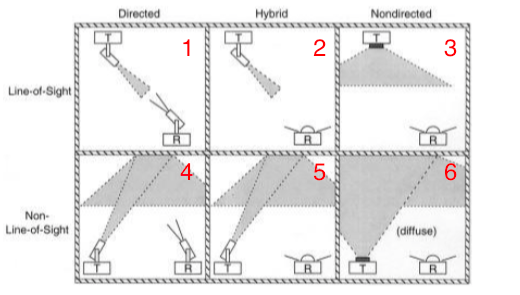
\includegraphics[width = 12cm]{figuras/difuso}
	\caption{Tipos de transmissão e recepção dos dados.}
	\label{Fig: difuso}
\end{figure}


Existem diversas maneiras de implementar um VLC fisicamente, os principais tipos são listados abaixo com diferentes combinações para cada categoria.
As transmissões podem ocorrer na linha de visão (\textit{Line-of-Sight}), como são os exemplos 1, 2 e 3 da figura [\ref{Fig: difuso}]. Este tipo de comunicação não conta com a reflexão do sinal em objetos ou obstáculos, cortando o link assim que algo interrompe a linha de comunicação direta.

Já as transmissões que contam com a reflexão do sinal para alcançar o receptor são chamados de fora da linha visão (\textit{Non-Line-of-Sight}) e mostrados nos quadros 4, 5 e 6 da figura [\ref{Fig: difuso}]. Tal tipo de configuração confere maior robustez ao sistema pelo fato de garantir a transmissão independente de obstáculos. Permitir que o link continue a operar mesmo com barreiras como pessoas ou móveis presente entre o transmissor e o receptor. Isto torna o uso do sistema mais fácil.

Em um sistema direcional, exemplificado nos quadros 1 e 4 da figura[\ref{Fig: difuso}]. Neste tipo de sistema o receptor Rx tem ângulo de recepção estreito, forçando que emissor e fotodetector tenham algum nível de alinhamento para permitir que a maior quantidade de potência seja transmitida, ou seja nesses sistemas temos uma elevada eficiência, quando comparada aos sistemas não direcionais pois a dispersão de luz é reduzida. Apesar de menos potência ser consumida isso não significa que o dispositivo será capaz de iluminar o ambiente por completo.
Em comparação os sistemas de não direcionais, eles tem ângulo de transmissão e recepção abertos, muito parecido com os LEDs comuns de prateleira. \cite{z.ghassemlooy2003}




